%%%%%%%%%%%%%%%%%%%%%%%%%%%%%%%%%%%%%%%%%
% Journal Article
% LaTeX Template
% Version 1.2 (15/5/13)
%
% This template has been downloaded from:
% http://www.LaTeXTemplates.com
%
% Original author:
% Frits Wenneker (http://www.howtotex.com)
%
% License:
% CC BY-NC-SA 3.0 (http://creativecommons.org/licenses/by-nc-sa/3.0/)
%
%%%%%%%%%%%%%%%%%%%%%%%%%%%%%%%%%%%%%%%%%

%----------------------------------------------------------------------------------------
%	PACKAGES AND OTHER DOCUMENT CONFIGURATIONS
%----------------------------------------------------------------------------------------

\documentclass[twoside]{article}

\usepackage{graphicx}

\usepackage{lipsum} % Package to generate dummy text throughout this template

\usepackage[sc]{mathpazo} % Use the Palatino font
\usepackage[T1]{fontenc} % Use 8-bit encoding that has 256 glyphs
\linespread{1.05} % Line spacing - Palatino needs more space between lines
\usepackage{microtype} % Slightly tweak font spacing for aesthetics

\usepackage[hmarginratio=1:1,top=32mm,columnsep=20pt]{geometry} % Document margins
\usepackage{multicol} % Used for the two-column layout of the document
\usepackage[hang, small,labelfont=bf,up,textfont=it,up]{caption} % Custom captions under/above floats in tables or figures
\usepackage{booktabs} % Horizontal rules in tables
\usepackage{float} % Required for tables and figures in the multi-column environment - they need to be placed in specific locations with the [H] (e.g. \begin{table}[H])
\usepackage{hyperref} % For hyperlinks in the PDF

\usepackage{lettrine} % The lettrine is the first enlarged letter at the beginning of the text
\usepackage{paralist} % Used for the compactitem environment which makes bullet points with less space between them

\usepackage{abstract} % Allows abstract customization
\renewcommand{\abstractnamefont}{\normalfont\bfseries} % Set the "Abstract" text to bold
\renewcommand{\abstracttextfont}{\normalfont\small\itshape} % Set the abstract itself to small italic text

\usepackage{titlesec} % Allows customization of titles
\renewcommand\thesection{\Roman{section}}
\titleformat{\section}[block]{\large\scshape\centering}{\thesection.}{1em}{} % Change the look of the section titles

\usepackage{fancyhdr} % Headers and footers
\pagestyle{fancy} % All pages have headers and footers
\fancyhead{} % Blank out the default header
\fancyfoot{} % Blank out the default footer
\fancyhead[C]{Flex Board Meets OBD $\bullet$ August 2013} % Custom header text
\fancyfoot[RO,LE]{\thepage} % Custom footer text

%----------------------------------------------------------------------------------------
%	TITLE SECTION
%----------------------------------------------------------------------------------------

\title{\vspace{-15mm}\fontsize{24pt}{10pt}\selectfont\textbf{Flex Board Meets OBD}} % Article title

\author{
\large
\textsc{Alessio Balsini}\\[2mm] % Your name
\textsc{David Librera}\\[2mm] % Your name
\normalsize Universit\`a degli Studi di Pisa\\ % Your institution
\normalsize Scuola Superiore Sant'Anna\\ % Your institution
\normalsize \href{mailto:a.balsini@sssup.it}{a.balsini@sssup.it} % Your email address
\normalsize \href{mailto:d.librera@sssup.it}{d.librera@sssup.it} % Your email address
\vspace{-5mm}
}
\date{}

%----------------------------------------------------------------------------------------

\begin{document}

\maketitle % Insert title

\thispagestyle{fancy} % All pages have headers and footers

%----------------------------------------------------------------------------------------
%	ABSTRACT
%----------------------------------------------------------------------------------------

\begin{abstract}

%\noindent \lipsum[1] % Dummy abstract text
\noindent The aim of the project is the development of a bridge made of a Flex Demo Board, a Bluetooth/UART module and an Elm327 device. The bridge gathers information from a standard OBDII vehicle and makes it available to other platforms.

\end{abstract}

%----------------------------------------------------------------------------------------
%	ARTICLE CONTENTS
%----------------------------------------------------------------------------------------

\begin{multicols}{2} % Two-column layout throughout the main article text

\section{Introduction}

\lettrine[nindent=0em,lines=2.5]{N} owadays almost all the vehicles adopt the OBDII standard. It allows the user not only to retrieve diagnostic data, but also to program the control units and modify vehicle's parameters in real time.

%------------------------------------------------

\section{Hardware}

\subsection{Connectors and Wirings}

The Flex Demo Board pins involved in the project are the following:

\begin{figure}[H]
  \centering
  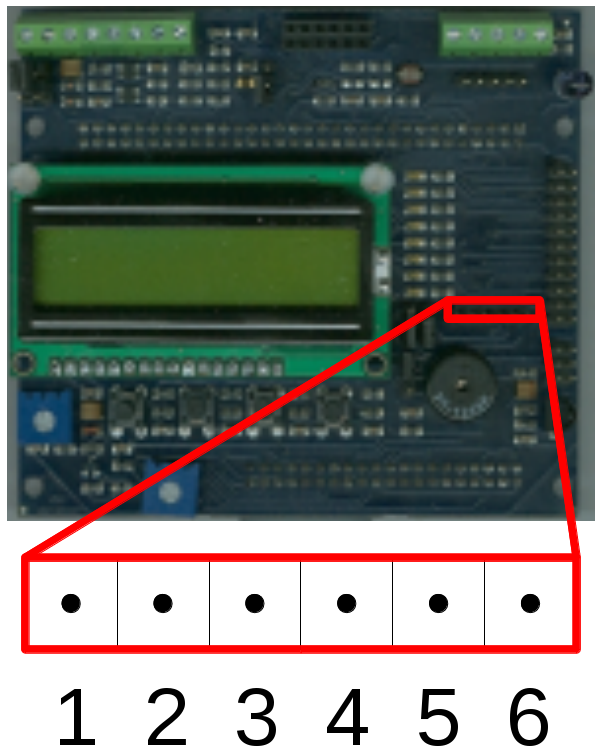
\includegraphics[width=2in]{img/flex_demo_board_pinout}
  \caption{\textit{Flex Demo Board} pinout}
\end{figure}

\begin{compactitem}
\item pin 1: 5 V;
\item pin 2: TX-O, UART output;
\item pin 3: SCK, Serial ClocK;
\item pin 4: RX-I, UART input;
\item pin 5: i.e. Vout;
\item pin 6: i.e. GND.
\end{compactitem}

The Bluetooth device uses has the following pinout:

\begin{figure}[H]
  \centering
  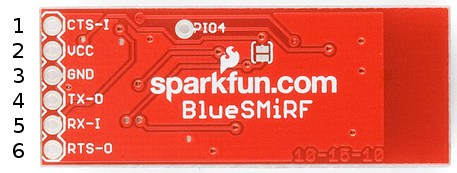
\includegraphics[width=3in]{img/bluesmirf_pinout}
  \caption{\textit{Bluesmirf} (Bluetooth/UART module) pinout}
\end{figure}

\begin{compactitem}
\item pin 1: CTS-I, Clear to Send (handshake pin);
\item pin 2: VCC (from 3.3V to 6V);
\item pin 3: GND;
\item pin 4: TX-O, UART output;
\item pin 5: RX-I, UART input;
\item pin 6: RTS-O, Request to Send (handshake pin).
\end{compactitem}

The Bluesmirf module has been connected to the Flex Demo Board with the following wiring:

\begin{compactitem}
\item Flex RX-I <-> Bt TX-O;
\item Flex TX-O <-> Bt RX-I;
\item Flex 5 V <-> Bt Vcc;
\item Flex GND <-> Bt GND.
\end{compactitem}

The standard OBDII female connector has the following pinout:

\begin{figure}[H]
  \centering
  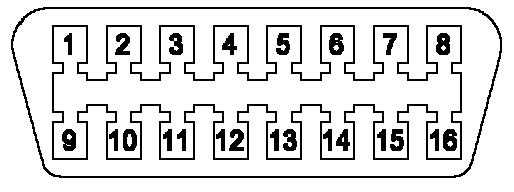
\includegraphics[width=2.5in]{img/J1962_female_pinout}
  \caption{OBD female connector pinout}
\end{figure}

\begin{compactitem}
\item pin 1: NC;
\item pin 2: Bus+ (J1850);
\item pin 3: NC;
\item pin 4: GND (chassis);
\item pin 5: GND (signal);
\item pin 6: CAN High (J-2284);
\item pin 7: K-Line (ISO9141-2);
\item pin 8: NC;
\item pin 9: NC;
\item pin 10: Bus (J1850);
\item pin 11: NC;
\item pin 12: NC;
\item pin 13: NC;
\item pin 14: CAN Low (J-2284);
\item pin 15: L-Line (ISO9141-2);
\item pin 16: Board Power (12 V).
\end{compactitem}


%------------------------------------------------

\section{Software}

\begin{table}[H]
\caption{Example table}
\centering
\begin{tabular}{llr}
\toprule
\multicolumn{2}{c}{Name} \\
\cmidrule(r){1-2}
First name & Last Name & Grade \\
\midrule
John & Doe & $7.5$ \\
Richard & Miles & $2$ \\
\bottomrule
\end{tabular}
\end{table}

\lipsum[5] % Dummy text

\begin{equation}
\label{eq:emc}
e = mc^2
\end{equation}

\lipsum[6] % Dummy text

%------------------------------------------------

\section{Manual}

%\lipsum[7-8] % Dummy text
\subsection{Wiring}

Wire the module like that.

\subsection{User Interaction}

Software starts with a welcome message...


%----------------------------------------------------------------------------------------
%	REFERENCE LIST
%----------------------------------------------------------------------------------------

\begin{thebibliography}{99} % Bibliography - this is intentionally simple in this template

\bibitem{} A. S. Huang, L. Rudolph,
  \emph{Bluetooth Essentials for Programmers},
  Cambridge University Press (2007)

\bibitem{}
  \emph{Bluetooth Data Module Command Reference \& Advanced Information User's Guide},
  Roving Networks (2013)

 
\end{thebibliography}

%----------------------------------------------------------------------------------------

\end{multicols}

\end{document}
